\documentclass[notes]{beamer}


\usepackage{pgfpages}
%\setbeameroption{show notes}
%\setbeameroption{show notes on second screen=right}
\mode<presentation> {
  \usetheme{Warsaw}
  % ou autre ...

  \setbeamercovered{transparent}
  % ou autre chose (il est également possible de supprimer cette ligne)
}


\usepackage[french]{babel}
\usepackage[latin1]{inputenc}
\usepackage{times}
\usepackage[T1]{fontenc}
\usepackage{tikz}
\usepackage[export]{adjustbox} %For aligining images left/right
\pgfdeclareimage[height=0.5cm]{le-logo}{logo_ujm}
\logo{\pgfuseimage{le-logo}}
\setbeamertemplate{footline}[frame number]


%%%%%%%%%%%%%%%%%%%%%%%%%%%
\title[Patterns for SoS Reconfiguration] 
{Automatic Sychronisation of Subtitle Track With Live Audio}
%\subtitle {ne compléter que si l'article possède un sous-titre}

\author[Joshua Fenech] 
%{F.~Petitdemange\inst{1} \and I.~Borne\inst{1} \and J.~Buisson\inst{2}}
{Joshua Fenech}

\institute[]
{
	MLDM\\
	Universit\'e de Jean Monnet\\
	Saint-\'Etienne, France
  %\inst{1}
  %IRISA\\
  %University of South Brittany\\
  %Vannes, France
  %\and
  %\inst{2}%
  %RISA\\
  %Military Academy of St-Cyr\\
  %Vannes, France
}

\date[SESOS 2015] 
{M1 Masters Thesis 2018}



\begin{document}


\begin{frame}
  \titlepage
\end{frame}


\section{Introduction}

\subsection{Introduction}

%---------------------------------------------------------------------------------------------------------------------

\begin{frame}{Problem Motivation}
\begin{figure}
	\centering
	\begin{minipage}{0.45\textwidth}
		\centering
		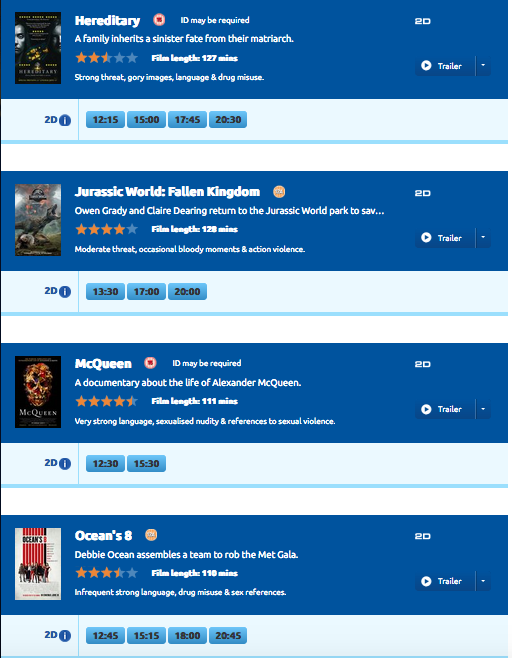
\includegraphics[width=0.9\textwidth]{figures/ALLMOVIESLONDONFULL} % first figure itself
		\caption{Full FIlm Showings 1 Day}
	\end{minipage}\hfill
	\begin{minipage}{0.45\textwidth}
		\centering
		%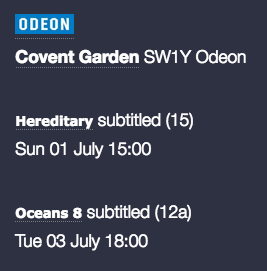
\includegraphics[width=0.9\textwidth]{figures/SUBSMOVIESLONDON} % second figure itself
		%\caption{second figure}
	\end{minipage}
\end{figure}
\end{frame}

%---------------------------------------------------------------------------------------------------------------------

\begin{frame}{Problem Motivation}
\begin{figure}
	\centering
	\begin{minipage}{0.45\textwidth}
		\centering
		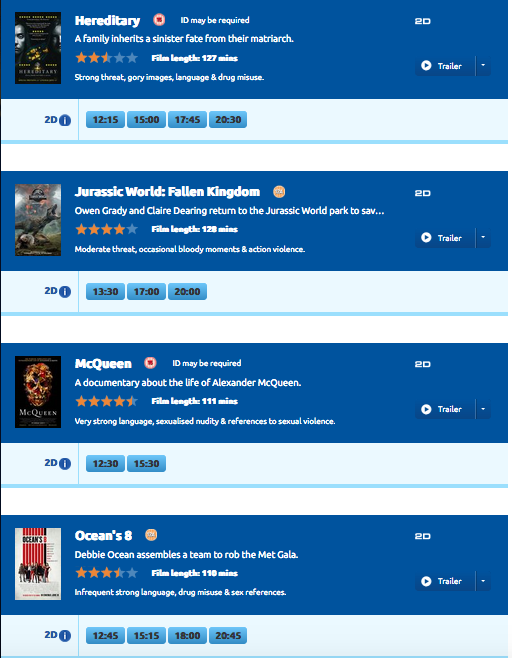
\includegraphics[width=0.9\textwidth]{figures/ALLMOVIESLONDONFULL} % first figure itself
		\caption{Full Film Showings 1 Day}
	\end{minipage}\hfill
	\begin{minipage}{0.45\textwidth}
		\centering
		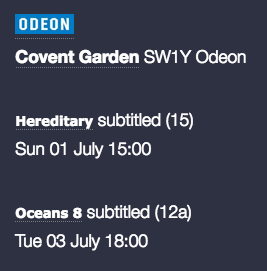
\includegraphics[width=0.9\textwidth]{figures/SUBSMOVIESLONDON} % second figure itself
		\caption{Subtitled FIlm Showings 1 Week}
	\end{minipage}
\end{figure}
\end{frame}

\note{
	\item Number of deaf people
	\item Deaf people feeling excluded
	\item Tourists
	}

%---------------------------------------------------------------------------------------------------------------------

\begin{frame}{Aim}
\begin{itemize}
	\item Develop a method to watch subtitles on a phone
	\item Problem: Synchronising the subtitles to the film
	\item Therefore, must identify the time in the film based on audio signals
\end{itemize}
\end{frame}

%---------------------------------------------------------------------------------------------------------------------

\begin{frame}{Prior Knowledge}
\begin{figure}
	\centering
	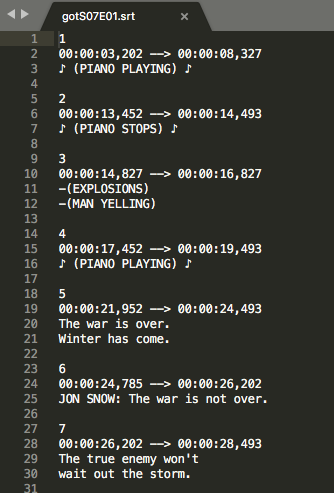
\includegraphics[width=0.5\textwidth]{figures/srt}
	\caption{SubRip .srt File}
\end{figure}
\begin{itemize}
	\item Subrip files contain list of entries indicating start time, stop time and text to be displayed
\end{itemize}
\end{frame}

\note{
	\item Who here has pirated a film?
	\item Used subtitles?
	\item srt
}

%---------------------------------------------------------------------------------------------------------------------

\begin{frame}{General Method}
\begin{itemize}
	\item Record audio, compressed using MP3
	\item Split signal into frames of duration 25ms - consider signal constant over this period
	\item Extract Mel Frequency Cepstral Coefficients (MFCC's)
	\item Use MFCC's as predictive feature of whether speech is present in a frame or not
	\item Match these predictions to the truth array, defined by a subtitle file
\end{itemize}
\end{frame}
%---------------------------------------------------------------------------------------------------------------------


\begin{frame}{Prior Knowledge}
\begin{itemize}
  \item How do you use subtitles on a laptop?
  \item SubRip Subtitle file (.srt)
\end{itemize}
\end{frame}

%---------------------------------------------------------------------------------------------------------------------

\begin{frame}{MP3 Compression}
\begin{figure}
	\centering
	\includegraphics[width=0.5\textwidth]{"figures/Frequency Response from Perceptual Coding of Digital Audio NOCAPTION"}
	\caption{Frequency respons of human hearing}
\end{figure}
\begin{itemize}
	\item Absolute threshold of hearing
	
\end{itemize}
\end{frame}

%---------------------------------------------------------------------------------------------------------------------

\begin{frame}{MFCC Audio Features}
\begin{minipage}{0.45\textwidth}
	\centering
	\begin{figure}
		\includegraphics[width=0.9\textwidth]{figures/MFCC_process}
		\caption{Sourced from}
	\end{figure}
	
\end{minipage}\hfill
\begin{minipage}{0.45\textwidth}
\begin{itemize}
	\item Process based on psychoacoustics to represent features most important to human hearing
	\item Split audio file into small sections, consider features constant over this period of time
	\item Apply a series of transformations
	\item Reduce stuff
\end{itemize}
\end{minipage}\hfill
\end{frame}

%---------------------------------------------------------------------------------------------------------------------

\begin{frame}{MFCC Audio Features}

	\centering
	\begin{figure}
		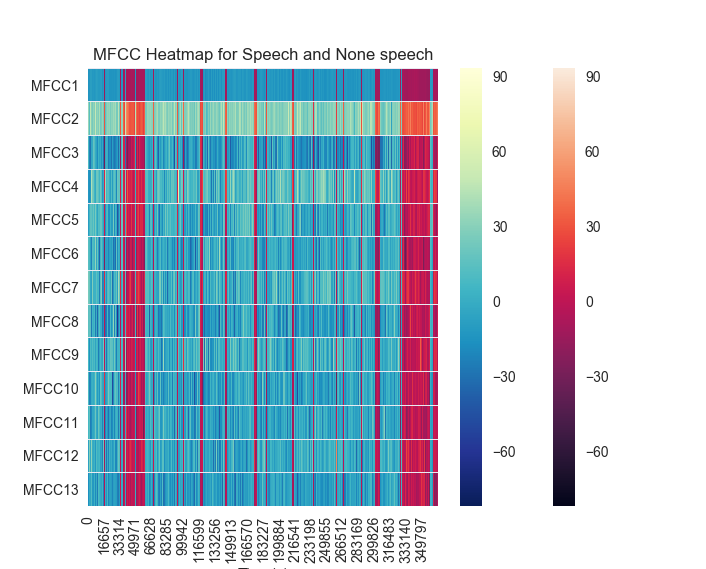
\includegraphics[width=0.7\textwidth]{figures/mfcc_heatmap_speech_or_nospeech}
		\caption{MFCC's Game of Thrones}
	\end{figure}

\end{frame}

%---------------------------------------------------------------------------------------------------------------------

\begin{frame}{Learner Architecture}
\begin{minipage}{0.45\textwidth}
	\begin{figure}
		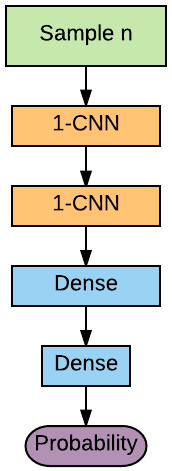
\includegraphics[width=0.5\textwidth]{figures/cnn_sabater}
		\caption{Model architecture}
	\end{figure}
\end{minipage}
\begin{minipage}{0.45\textwidth}
	\begin{figure}
		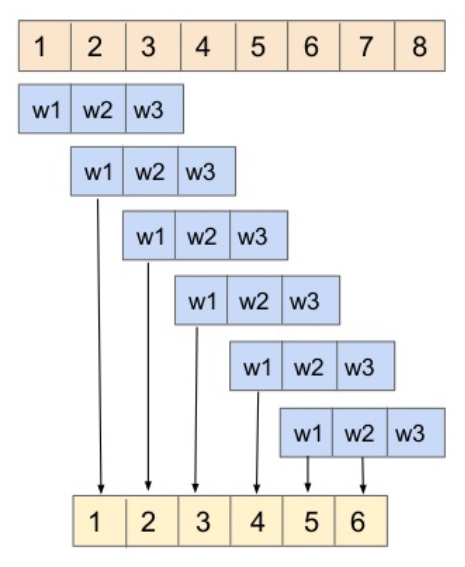
\includegraphics[width=0.7\textwidth]{figures/1dconv_nopad}
		\caption{1d convolutions, no padding}
	\end{figure}
	
\end{minipage}
\end{frame}

%---------------------------------------------------------------------------------------------------------------------

\begin{frame}{Results}
\begin{itemize}
	\item Learner trained on Game of Thrones episode
	\item Results on validation data suggested this was sufficient
\end{itemize}
\end{frame}

%---------------------------------------------------------------------------------------------------------------------

\begin{frame}{Synchronisation}
\begin{itemize}
	\item Access to dataset granted incrementally as new audio is recorded
	\item Initially attempted to match a window of predicted probabilities with a similar array generated from srt
	\item Problem: Beginning of film often has no subtitle
	\item Solution: Continue recording data until speech is detected, and identify this as start of subtitle track
\end{itemize}
\end{frame}




\end{document}